\chapter{Software Test Plan}
\section{Inleiding}
Het systeem kan op verschilende manieren getest worden. 
Langs de ene kant zijn er tests voor onafhankelijke stukken code (Unittests), en langs de andere kant wordt de samenwerking van deze componenten getest (Integratietests). 
Daarnaast moet op vlak van GUI getest worden of de applicatie stabiel blijft in bepaalde scenario's, of bij foute input. 
Door middel van tests moet gegarandeerd worden dat het systeem werkt en voldoet aan de specificaties beschreven in het SRS\cite{srs}. 
Wanneer de programmeur code wenst te pushen naar de hoofdrepository moet deze eerst alle tests successvol uitvoeren. 
Wanneer voldoende tests zijn geschreven garandeert dit dat het systeem werkt zoals verwacht.

\section{Soorten tests}

\subsection{Unittests}
Unittests zijn tests die kleine, onafhankelijke stukken code testen. Code die door unittests getest wordt mag geen gebruik maken van externe bronnen, anders kan men niet nagaan of de fout in de te testen klasse/methode zit, of in de externe code.
Wanneer een klasse wordt afgewerkt (of een subset van zijn methoden) moet hiervoor reeks unittests worden geschreven. 
Deze tests moeten correctheid van een individueel component nagaan. 
Wanneer de klasse wordt aangepast kunnen deze tests opnieuw gerunt worden. Hierdoor kunnen mogelijke problemen vroeg gedetecteerd worden.
Deze tests bevatten o.a. ook tests over de database, die vaak als een aparte categorie worden beschouwd. 

\subsection{Integratietests}
Bij unittests werd vermeld dat de klassen geen gebruik mogen maken van externe bronnen. Wanneer dit wel zo is, en dus de samenwerking tussen de twee componenten wordt getest, zijn dit integratietests, m.a.w. hoe twee of meer componenten met elkaar integreren. 
Gewoonlijk vangen integratietests meer bugs en regressies dan unittests, daarom moet de programmeur extra aandacht besteden aan het schrijven van dit soort tests.

\subsection{Verificatietests}
Verificatietests testen en garanderen dat het systeem voldoet aan de requirements beschreven in het SRS\cite{srs}. 
Deze tests zijn niet mutueel exclusief met unittests en integratietests, maar zijn in sommige gevallen wel expliciet nodig.

\subsection{GUI tests}
De GUI wordt ook uitvoerig getest. Deze moet blijven werken zoals verwacht met arbitraire input. Deze tests worden eveneens geautomatiseerd.

\section{Tools}
Door middel van JUnit 4\cite{junit} worden tests opgesteld voor het project. 
JUnit is een standaard Java library en overigens geïntegreerd in de user interface van Eclipse, waardoor het uitvoeren van tests makkelijk wordt en zodat men makkelijk conclusies kan trekken nadat alle tests gerunt zijn. 
Met JUnit kunnen makkelijk tests geschreven worden d.m.v. ``assertions''. 
Een assertion test of een echte waarde (verkregen door het uitvoeren van een methode) gelijk is aan de verwachte waarde opgegeven door de programmeur. Wanneer dit het geval is faalt de test. 	

\section{Criteria voor succesvolle tests}
Wanneer er geen fouten gevonden worden in een klasse d.m.v. de bijhorende tests zeggen we dat deze slaagt. 
Indien er zich wel fouten voordoen moeten deze worden opgelost alvorens de code mag worden opgenomen in de hoofdrepository.
De programmeur die een fout omerkt maakt steeds een issue aan op GitHub indien hij zelf niet verantwoordelijk is voor de falende code.
Deze bug reports worden toegewezen aan de verantwoordelijke voor de falende code, welke de code zo snel mogelijk moet verbeteren. 
Wanneer een test faalt in onverwachte omstandigheden, m.a.w. in code die de programmeur niet heeft aangepast maar eventueel wel gebruikt, moet hiervoor ook een issue geplaatst worden op GitHub.

\noindent
Deze issue bevat de volgende informatie:
\begin{itemize}
	\item Het requirement ID, zoals gespecifieerd in het SRS\cite{srs}
	\item Een beschrijving van het probleem
	\item Input die het probleem veroorzaakt
	\item De verwachte output
	\item De daadwerkelijke output
\end{itemize}

Deze issue kan daarna opgelost worden door de programmeur verantwoordelijk voor de falende code, of door bijdrage van andere programmeurs.

\section{Verantwoordelijkheden}
De programmeur is verantwoordelijk voor het schrijven van tests voor zijn afgewerkte onderdelen. Code waar geen tests voor geschreven zijn mag niet worden opgenomen in de hoofdrepository op GitHub. Zonder tests kan de werking van deze code eenmaal niet worden bevestigd. De Software Quality Assurance Manager is verantwoordelijk voor het controleren dat de programmeurs deze tests volledig en correct schrijven.

\section{Indeling}
Alle tests worden bijgehouden in een aparte source folder in het project, genaamd \emph{src/main/tests}.
De directorystructuur in deze folder is dezelfde als die van de source code van het project.
Bronbestanden zijn georganiseerd in packages, en dat is met tests exact hetzelfde, maar met een \emph{.tests} suffix.
De java-klasse bronbestanden krijgen het \emph{Tests} suffix.

\noindent
Hier is één groep tests beschikbaar, nl. de tests die horen bij het bronbestand \emph{User.java} in het package \emph{com.vub.model}. 
De eigenlijke tests op dit bestand staan in de directory \emph{src/main/tests}. 
De bijhorende package noemt \emph{com.vub.model.tests}, met bestandsnaam \emph{UserTests.java} voor de tests.

\begin{figure}[ht!]
\centering
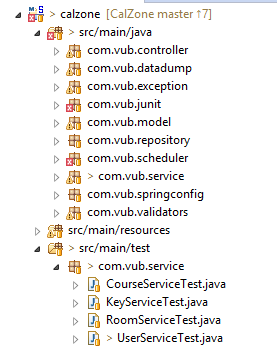
\includegraphics[width=90mm]{img/dir.png}
\caption{Directorystructuur van testbestanden.}
\label{dirstruct}
\end{figure}

\section{Belangrijkste Java code conventies}
\subsection{Naming conventions}
	\subsubsection{Klassen \& interfaces}
		Gebruik simpele, maar beschrijvende namen (zelfstandige naamwoorden) die iets zeggen over de klasse. Elk zelfstandig woord in de klassenaam begint met een hoofdletter. Vermijd acroniemen, tenzij deze algemeen gebruikt worden (zoals URL en HTTP).
		\\ \\
		\emph{\textbf{class Course;}} \\
		\emph{\textbf{class ProfilePageController;}}
		
	\subsubsection{Methoden}
		Namen van methoden beginnen met werkwoord (en een lowercase letter), met hoofdletters voor elk volgend woord.
		\\ \\
		\emph{\textbf{run();}} \\
		\emph{\textbf{runTests();}} \\
		\emph{\textbf{runTestInBackground();}}
		
	\subsubsection{Variabelen}
		Variabelen beginnen met een lowercase letter, met opeenvolgende woorden gestart worden met een hoofdletter. 
		De naam van een variabele moet kort, maar toch beschrijvend zijn. 
		De namen van constante variabelen in een klasse zijn volledig uppercase, met opeenvolgende woorden gescheiden door een underscore.
		\\ \\		
		\emph{\textbf{float width;}} \\
		\emph{\textbf{float minWidth;}} \\
		\emph{\textbf{int MIN\_WIDTH $=$ 1;}} \\
		\emph{\textbf{boolean DEBUG $=$ false;}} \\
		
		Bovendien wordt ook één declaratie per lijn aangemoedigd, omdat dit het schrijven van commentaar kan aanmoedigen.
		\\ \\
		\emph{\textbf{float width, height;} // fout} \\
		\emph{\textbf{float width;} // Width of the bridge} \\
		\emph{\textbf{float height;} // Height of the bridge}
		

\subsection{Klasse en interface declaraties}
	\begin{itemize}
		\item{Bij aanroep van een methode, geen spatie tussen de methode naam en het openende haakje}
		\item{De open brace \"\{\" staat op dezelfde lijn als de naam van de declaratie}
		\item{De sluitende brace staat automatisch op een nieuwe regel, tenzij de methode een lege body heeft}
		\item{Methoden zijn gescheiden door een blanke regel}
	\end{itemize}
	Voor elke klasse staat een comment met het volgende template:
	\\
	\\
	\emph{/*} \\
	\emph{ * Klasse naam} \\
	\emph{ *} \\
	\emph{ * Versie info} \\
	\emph{ *} \\
	\emph{ * Auteur} \\
	\emph{ *} \\
	\emph{ * Beschrijving van de klasse} \\
	\emph{*/} 